% !TEX program = xelatex
% Versão breve (5-8 páginas) – compilar com XeLaTeX (xelatex artigo_breve.tex, duas vezes)
\documentclass[12pt,a4paper]{article}
\usepackage{fontspec}
\setmainfont{TeX Gyre Termes}
\usepackage{polyglossia}
\makeatletter
\ifcsname l@portuges\endcsname\else\expandafter\let\csname l@portuges\endcsname\l@english\fi
\ifcsname l@portuguese\endcsname\else\expandafter\let\csname l@portuguese\endcsname\l@english\fi
\makeatother
\setdefaultlanguage[variant=brazilian]{portuguese}
\usepackage[top=3cm,left=3cm,bottom=2cm,right=2cm]{geometry}
\usepackage{setspace}
\onehalfspacing
\usepackage{indentfirst}
\setlength{\parindent}{1.25cm}
\setlength{\parskip}{0pt}
\emergencystretch=1.5em
\usepackage{amsmath}
\usepackage{graphicx}
\graphicspath{{figuras/}}
\usepackage{float}
\renewcommand{\topfraction}{0.95}\renewcommand{\bottomfraction}{0.95}
\renewcommand{\textfraction}{0.05}\renewcommand{\floatpagefraction}{0.85}
\setlength{\textfloatsep}{8pt plus 2pt minus 2pt}\setlength{\intextsep}{8pt plus 2pt minus 2pt}
\usepackage{booktabs}
\usepackage{etoolbox}\AtBeginEnvironment{tabular}{\singlespacing}
\usepackage{array}
\usepackage{caption}
\captionsetup{font=small,labelsep=endash,justification=centering,skip=4pt}
\usepackage{titlesec}
\titleformat{\section}{\normalsize\bfseries}{\thesection}{1em}{\MakeUppercase}
\titleformat{\subsection}{\normalsize}{\thesubsection}{1em}{\MakeUppercase}
\titlespacing*{\section}{0pt}{12pt}{8pt}
\titlespacing*{\subsection}{0pt}{8pt}{8pt}
\usepackage{fancyhdr}
\setlength{\headheight}{14pt}
\pagestyle{fancy}
\fancyhf{}
\fancyhead[R]{\small\thepage}
\renewcommand{\headrulewidth}{0pt}
\usepackage[hidelinks]{hyperref}
\urlstyle{same}
\newcommand{\fonte}[1]{\par\vspace{2pt}{\centering\small #1\par}\vspace{2pt}}
\newenvironment{referencias}{\begin{singlespace}\setlength{\parindent}{0pt}\setlength{\parskip}{4pt}\raggedright\footnotesize}{\end{singlespace}}

\begin{document}
\thispagestyle{empty}
\begin{singlespace}
\begin{center}
\textbf{ALTO VALOR ADICIONADO NA INDÚSTRIA, NOS SERVIÇOS E NA ADMINISTRAÇÃO PÚBLICA: GUAMARÉ, NATAL E CEARÁ-MIRIM À LUZ DA LITERATURA SOBRE DESENVOLVIMENTO SOCIOECONÔMICO}
\end{center}
\vspace{8pt}
\begin{flushright}
Iuri Guerra de Freitas Pereira\footnote{Pós-graduando em Ciência de Dados pelo Instituto Federal de Educação, Ciência e Tecnologia do Rio Grande do Norte (IFRN). Engenheiro de Computação, Mestre em Tecnologia da Informação. E\mbox{-}mail: \url{iuri.pereira@escolar.ifrn.edu.br}.}
\end{flushright}
\vspace{8pt}
\noindent\textbf{RESUMO}

\noindent O artigo identifica fatores associados ao alto Valor Adicionado Bruto (VAB) da indústria, dos serviços e da administração pública nos municípios do Rio Grande do Norte em 2021, último ano com abertura setorial do VAB municipal, e dialoga com a literatura sobre desenvolvimento socioeconômico. Com dados do IBGE, do IpeaData e do Observatório Sebrae para os 167 municípios, aplicam-se média, desvio padrão, percentis 10 e 90 e a reta $Y = a + bX$, lida em gráficos de dispersão; diagramas de caixa situam cada município na distribuição do seu setor. Os casos são Guamaré, Natal e Ceará-Mirim, escolhidos por VAB absoluto, participação, população e literatura disponível; Pau dos Ferros, João Dias e São Bento do Norte são avaliados como alternativas. Os municípios abaixo do percentil 10 do PIB per capita têm a administração pública como maior setor e os acima do percentil 90 têm a indústria, mas o IDHM mediano dos dois grupos é quase o mesmo. O diálogo com Mendes \textit{et al.} (2018) e Fernandes, Tavares e Azevedo (2018) confirma que VAB e PIB caminham juntos e contesta, para o caso potiguar, que a indústria seja o setor mais ligado ao desenvolvimento humano.

\vspace{4pt}
\noindent\textbf{Palavras-chave:} valor adicionado bruto; estatística descritiva; desenvolvimento socioeconômico; Rio Grande do Norte.
\end{singlespace}

\section{Introdução}

Em 2021 o Rio Grande do Norte gerou um Valor Adicionado Bruto de R\$ 71,06 bilhões, dos quais 45,5\% nos serviços, 29,4\% na administração pública e 20,7\% na indústria (IBGE, 2023). Quando se analisa município a município, o retrato é outro: a administração pública é o setor de maior VAB em 122 dos 167 municípios (73,1\%), e Natal, Mossoró e Parnamirim concentram 48,8\% do PIB e 63,7\% do VAB dos serviços. A indústria de maior peso está no litoral norte, em municípios pequenos ligados ao petróleo, ao gás, ao sal e à energia eólica (IBGE, 2023).

Este artigo aplica estatística descritiva qualitativa e quantitativa aos 167 municípios do RN no ano de 2021 (último ano com VAB municipal aberto por setor), seleciona um município com alto VAB em cada setor e dialoga com o estado da arte (Mendes et al., 2018; Fernandes, Tavares e Azevedo, 2018) para concordar ou divergir de seus achados sobre a relação entre estrutura produtiva e desenvolvimento socioeconômico.

O texto segue em quatro seções: dados, ferramentas e lacunas (seção 2); resultados, com a escolha de Guamaré, Natal e Ceará-Mirim para a indústria, os serviços e a administração pública e a avaliação de Pau dos Ferros, João Dias e São Bento do Norte como alternativas (seção 3); diálogo com dois artigos (seção 4); e considerações finais (seção 5).

\section{Dados e ferramentas}

A base reúne, para os 167 municípios, o PIB e o VAB por setor de 2002 a 2021 (IBGE, tabela 5938 do SIDRA), a população, os indicadores sociais e as receitas do IBGE Cidades, o pessoal ocupado do Cadastro Central de Empresas (CEMPRE) e os estabelecimentos ativos do Observatório Sebrae; os valores a preços de 2010 vêm do IpeaData. O VAB é a diferença entre o valor da produção de uma atividade e o consumo intermediário; o PIB municipal é a soma do VAB das atividades mais os impostos sobre produtos, e o PIB per capita divide esse total pela população:
\begin{equation}
\mathrm{PIB}_m = \sum_{s} \mathrm{VAB}_{m,s} + \mathrm{Imp}_m, \qquad
\mathrm{PIB\,pc}_m = \frac{\mathrm{PIB}_m}{\mathrm{Pop}_m} = \sum_{s} \frac{\mathrm{VAB}_{m,s}}{\mathrm{Pop}_m} + \frac{\mathrm{Imp}_m}{\mathrm{Pop}_m},
\end{equation}
em que $m$ é o município, $s$ a atividade, $\mathrm{Imp}$ os impostos líquidos sobre produtos e $\mathrm{Pop}$ a população estimada de 2021. As duas leituras de ``alto VAB'' usadas adiante derivam da mesma identidade:
\begin{equation}
\mathrm{Part}_{m,s} = 100 \cdot \frac{\mathrm{VAB}_{m,s}}{\sum_{s} \mathrm{VAB}_{m,s}}, \qquad
\mathrm{VAB\,pc}_{m,s} = \frac{\mathrm{VAB}_{m,s}}{\mathrm{Pop}_m}.
\end{equation}
A participação mede especialização e não depende do tamanho do município; o VAB por habitante é a parcela do PIB per capita gerada pelo setor, de modo que um setor com VAB por habitante alto eleva o PIB per capita mesmo em município pequeno. O IBGE estima o VAB de cada atividade no estado e o reparte entre os municípios por indicadores como a produção de petróleo, as saídas de mercadorias e a folha das prefeituras (IBGE, 2016): por isso ``Indústria'' inclui petróleo, refino, sal e energia elétrica, e o VAB da administração pública dos municípios pequenos reflete a folha da prefeitura, financiada em grande parte pelo FPM (Fundo de Participação dos Municípios).

Foram utilizadas as ferramentas estatísticas descritivas e inferenciais. A média $\bar{x}$ e o desvio padrão $s$ descrevem o centro e a variação dos dados; onde a soma dos quadrados dos desvios é mínima em relação à média, e $s$ é a raiz dessa soma dividida por $n-1$. Os percentis 10 (P10) e 90 (P90) do PIB per capita isolam os 10\% mais pobres e os 10\% mais ricos. A função afim $Y = a + bX$ relaciona duas variáveis em um gráfico de pontos; seus parâmetros minimizam a soma dos quadrados das distâncias verticais $y_i - (a + b x_i)$ entre cada ponto e a reta, o que resulta em
\begin{equation}
b = \frac{\sum (x_i - \bar{x})(y_i - \bar{y})}{\sum (x_i - \bar{x})^2}, \qquad a = \bar{y} - b\,\bar{x}.
\end{equation}

A associação entre duas variáveis é lida no gráfico de dispersão: se a reta sobe, os municípios acima da média em $X$ tendem a estar acima da média em $Y$; se é horizontal, não há associação linear; se desce, as variáveis caminham em sentidos opostos. O espalhamento dos pontos em torno da reta diz quanto ela resume os dados. O coeficiente de correlação de Pearson condensa inclinação e espalhamento em um número entre $-1$ e $+1$; foi dispensado porque, com três pares de padrão visual nítido (Figura \ref{fig:idhm}), a leitura da reta basta para a dedução. Para situar um município na distribuição do seu setor usa-se o diagrama de caixa: a caixa vai do primeiro ao terceiro quartil, a linha interna é a mediana, as hastes alcançam os pontos a até 1,5 caixa de distância e os demais são extremos; a média e o desvio padrão são marcados ao lado (Figura \ref{fig:box}). Salvo o IDHM, todas as variáveis de comparação são de 2021.

\subsection{Lacunas dos dados}

Quatro lacunas condicionam a leitura. (i) \textbf{Corte temporal do VAB setorial:} o último ano com VAB municipal aberto por setor no SIDRA é 2021; para 2022 e 2023 o IBGE divulgou apenas o PIB total, por isso toda a análise setorial para em 2021. (ii) \textbf{Anos diferentes entre indicadores:} o IDHM e a proporção de pessoas com renda de até meio salário mínimo são do Censo 2010, onze anos antes do VAB, e são os mais recentes disponíveis por município no IBGE Cidades na data da extração (9 out. 2026); o emprego formal é do CEMPRE 2021 e as receitas, de 2025. Associar o VAB de 2021 a um indicador de 2010 ou de 2025 supõe que a posição relativa dos municípios mudou pouco no período, hipótese plausível para o IDHM, cuja ordenação é estável, e mais frágil para as receitas. (iii) \textbf{Classificação setorial:} ``Serviços'' no IBGE exclui a administração pública mas inclui o comércio, e ``Administração pública'' inclui educação, saúde e seguridade públicas; estudos nacionais que somam os dois grupos chegam a sinais diferentes (seção 4.3). (iv) \textbf{Municípios pequenos e enclaves:} 50 dos 167 municípios têm menos de 5 mil habitantes, e uma única planta de petróleo, sal ou energia eólica infla o VAB por habitante; em Guamaré o VAB industrial foi negativo entre 2011 e 2014 e o VAB total, em 2012 e 2013, o que torna a participação setorial desses anos indefinida. A mortalidade infantil, ausente para a maioria dos municípios pequenos, ficou de fora.

\section{Resultados}

A Tabela \ref{tab:p} resume o padrão mais claro dos dados. Os 17 municípios com PIB per capita até o P10 (R\$ 10.039) têm, todos, a administração pública como maior setor, com mediana de 67,1\% do VAB, 5,3\% da população em emprego formal e 93,3\% da receita vinda de transferências. Os 17 a partir do P90 (R\$ 29.137) são, em 15 casos, municípios de indústria. O IDHM mediano, porém, é 0,587 no grupo pobre, 0,608 no grupo do meio e 0,605 no grupo rico: ser muito rico em PIB per capita está associado a ter indústria, não a ter melhor desenvolvimento humano.

\begin{table}[!htb]
\centering
\caption{Medianas dos grupos definidos pelos percentis 10 e 90 do PIB per capita, 2021}
\label{tab:p}
\footnotesize
\begin{tabular}{@{}p{6.2cm}>{\centering\arraybackslash}p{2.4cm}>{\centering\arraybackslash}p{2.9cm}>{\centering\arraybackslash}p{2.6cm}@{}}
\toprule
Indicador (mediana do grupo) & Até P10 \newline (n = 17) & Entre P10 e P90 \newline (n = 133) & A partir de P90 \newline (n = 17) \\
\midrule
PIB per capita 2021 (R\$) & 9.545 & 13.469 & 47.183 \\
Part. Adm. pública no VAB (\%) & 67,1 & 51,7 & 17,1 \\
Part. Indústria no VAB (\%) & 4,2 & 5,1 & 59,4 \\
Part. Serviços no VAB (\%) & 22,8 & 27,5 & 13,9 \\
Transferências na receita 2025 (\%) & 93,3 & 91,2 & 89,3 \\
\% pop. em emprego formal 2021 & 5,3 & 8,2 & 13,0 \\
IDHM 2010 & 0,587 & 0,608 & 0,605 \\
\bottomrule
\end{tabular}
\fonte{Fonte: elaborada pelo autor (2026) com dados do IBGE (2023), IBGE Cidades e CEMPRE.}
\end{table}

A Figura \ref{fig:sep} mostra as separatrizes: os 167 municípios em ordem crescente de PIB per capita, as linhas do P10 e do P90 e cada ponto colorido pelo setor de maior VAB. Abaixo do P10 todos os pontos são de administração pública; entre o P10 e o P90 ela continua dominante, com serviços e indústria aparecendo só perto do P90; acima do P90, 15 dos 17 municípios são de indústria. A Figura \ref{fig:dom} mostra que esse domínio é estrutural: a administração pública é o maior VAB em 122 municípios em 2021, contra 22 da indústria e 20 dos serviços (nos 3 restantes nenhum dos três setores é o maior), e já era em 137 em 2002; a queda de 15 municípios em vinte anos foi absorvida pelos serviços, que passaram de 7 para 20.

\begin{figure}[!htb]
\centering
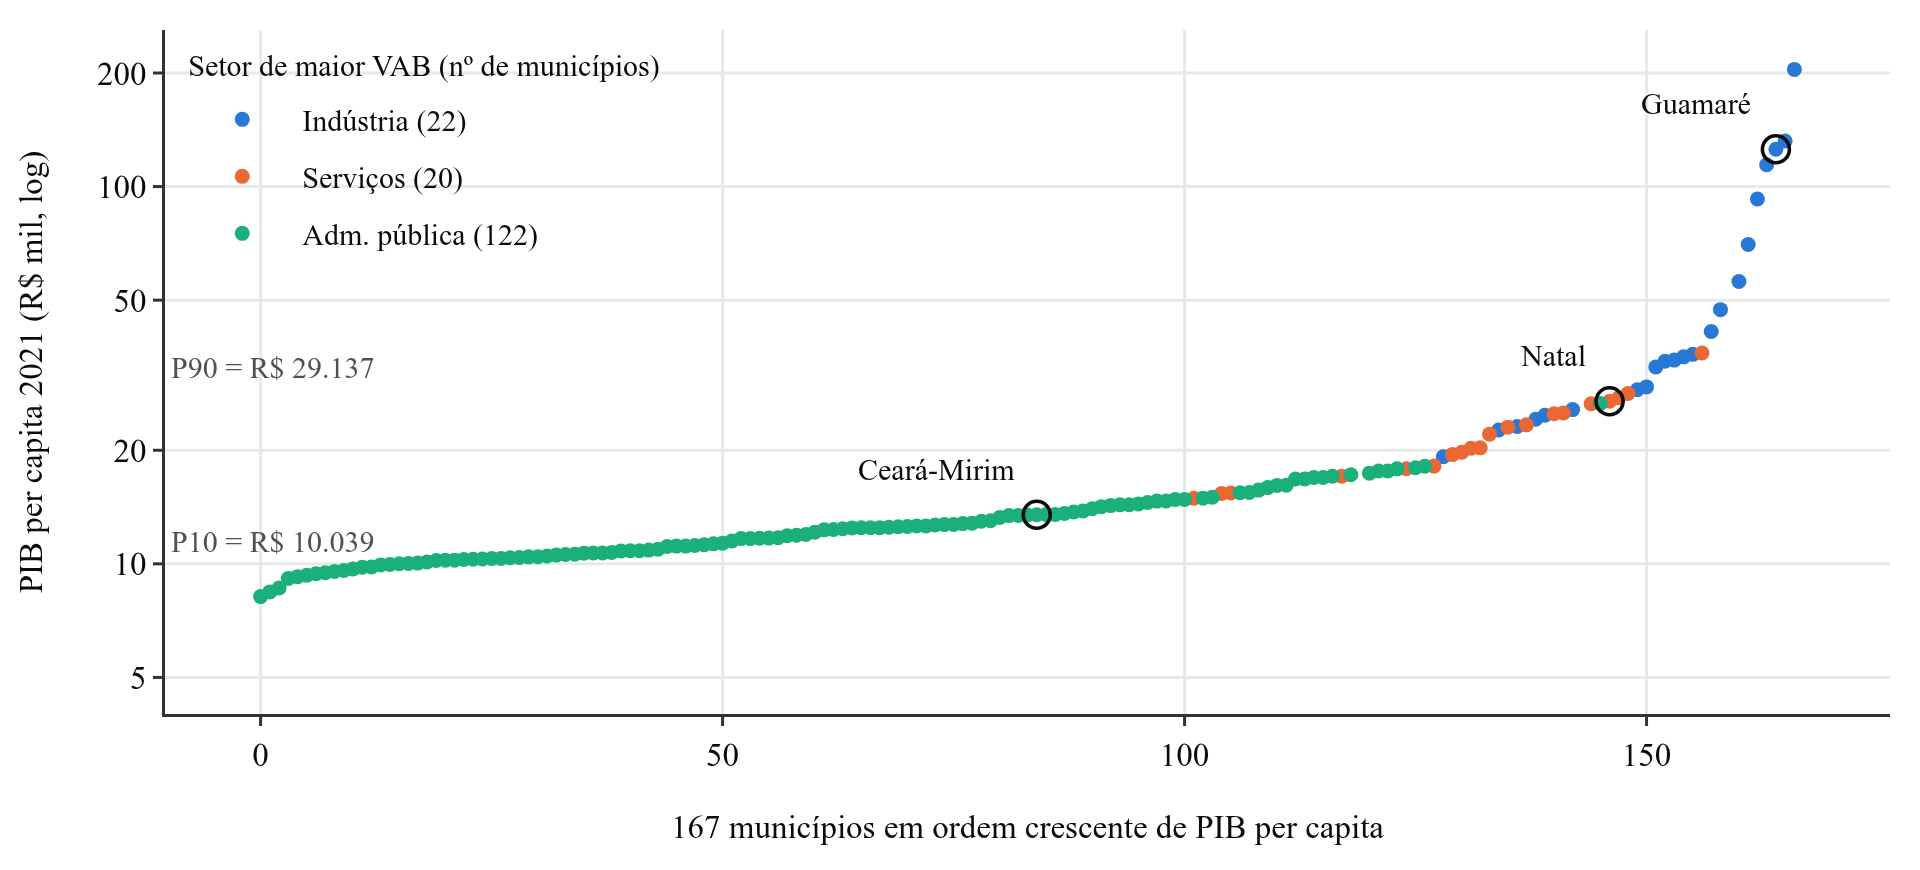
\includegraphics[width=0.85\textwidth]{fig2_separatrizes.png}
\caption{PIB per capita de 2021 dos 167 municípios em ordem crescente, com os percentis 10 e 90 e o setor de maior VAB de cada município (omitidos os 3 municípios em que nenhum dos três setores é o maior)}
\label{fig:sep}
\fonte{Fonte: elaborada pelo autor (2026) com dados do IBGE (2023).}
\end{figure}
\begin{figure}[!htb]
\centering
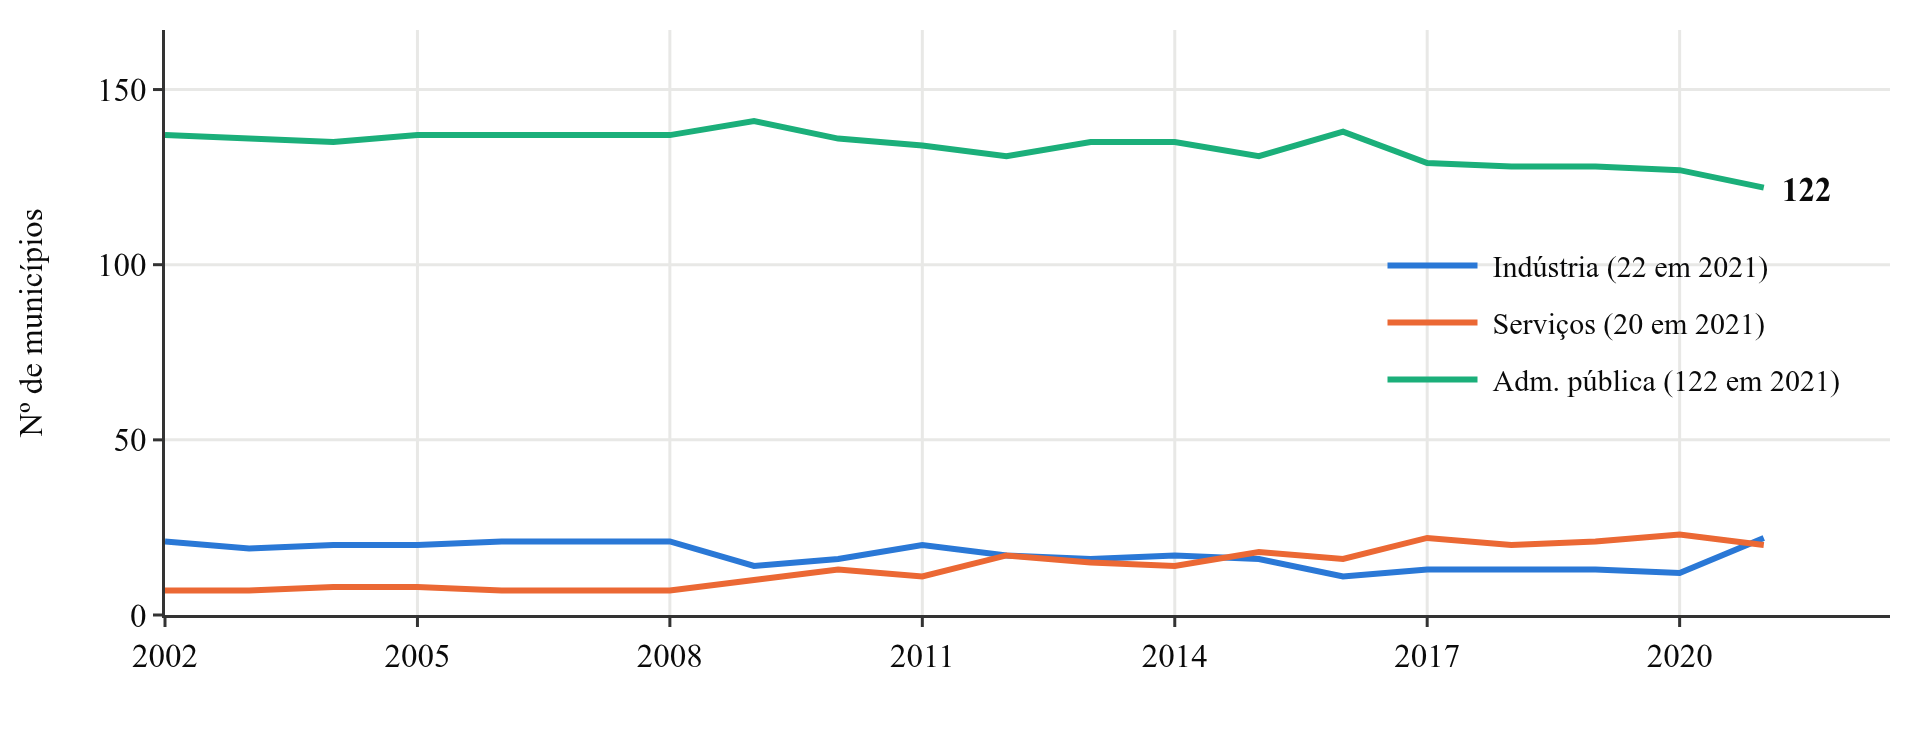
\includegraphics[width=0.8\textwidth]{fig3_setor_dominante.png}
\caption{Número de municípios em que cada um dos três setores é o maior VAB, 2002--2021}
\label{fig:dom}
\fonte{Fonte: elaborada pelo autor (2026) com dados do IBGE (2023).}
\end{figure}

A Figura \ref{fig:idhm} compara a participação de cada setor com o IDHM, com a reta $Y = a + bX$ ajustada aos 167 municípios e o município escolhido do setor em destaque. Na indústria a reta é horizontal ($b = -0{,}003$ de IDHM por 100 pontos percentuais): Guamaré, com 75\% do VAB na indústria, tem IDHM 0,015 acima da média, e os municípios mais industriais do estado estão abaixo dela. Nos serviços a reta sobe ($b = +0{,}208$) e Natal é o extremo das duas variáveis. Na administração pública a reta desce ($b = -0{,}071$) e Ceará-Mirim está sobre a média nos dois eixos. A Figura \ref{fig:inv} mostra a relação inversa de outro modo, agrupando os municípios pelo setor de maior VAB: nos 122 em que a administração pública domina, o IDHM mediano é 0,603 e 7,5\% da população tem emprego formal; nos 20 de serviços, 0,653 e 13,0\%; nos 22 de indústria, 0,592 e 9,8\%. Onde a prefeitura é a maior atividade econômica, o desenvolvimento humano é menor e o trabalho é mais informal; onde a indústria domina, a renda é alta, mas o IDHM mediano é o pior dos três grupos.

\begin{figure}[!htb]
\centering
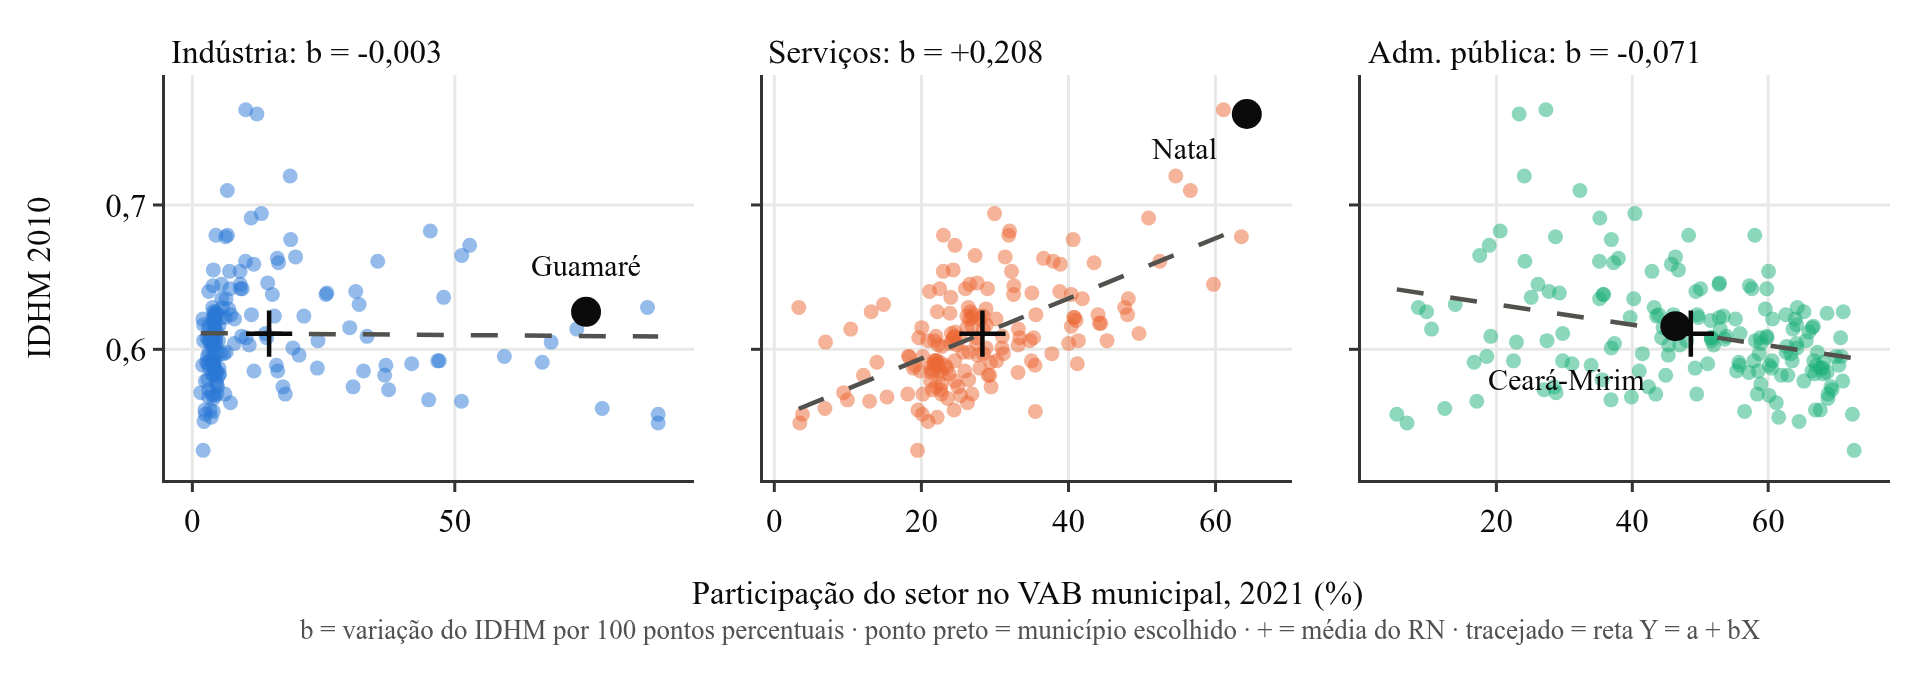
\includegraphics[width=\textwidth]{fig4_setores_idhm.png}
\caption{Participação de cada setor no VAB municipal (2021) contra o IDHM (2010), 167 municípios: reta $Y = a + bX$, média do RN e município escolhido}
\label{fig:idhm}
\fonte{Fonte: elaborada pelo autor (2026) com dados do IBGE (2023) e IBGE Cidades.}
\end{figure}
\begin{figure}[!htb]
\centering
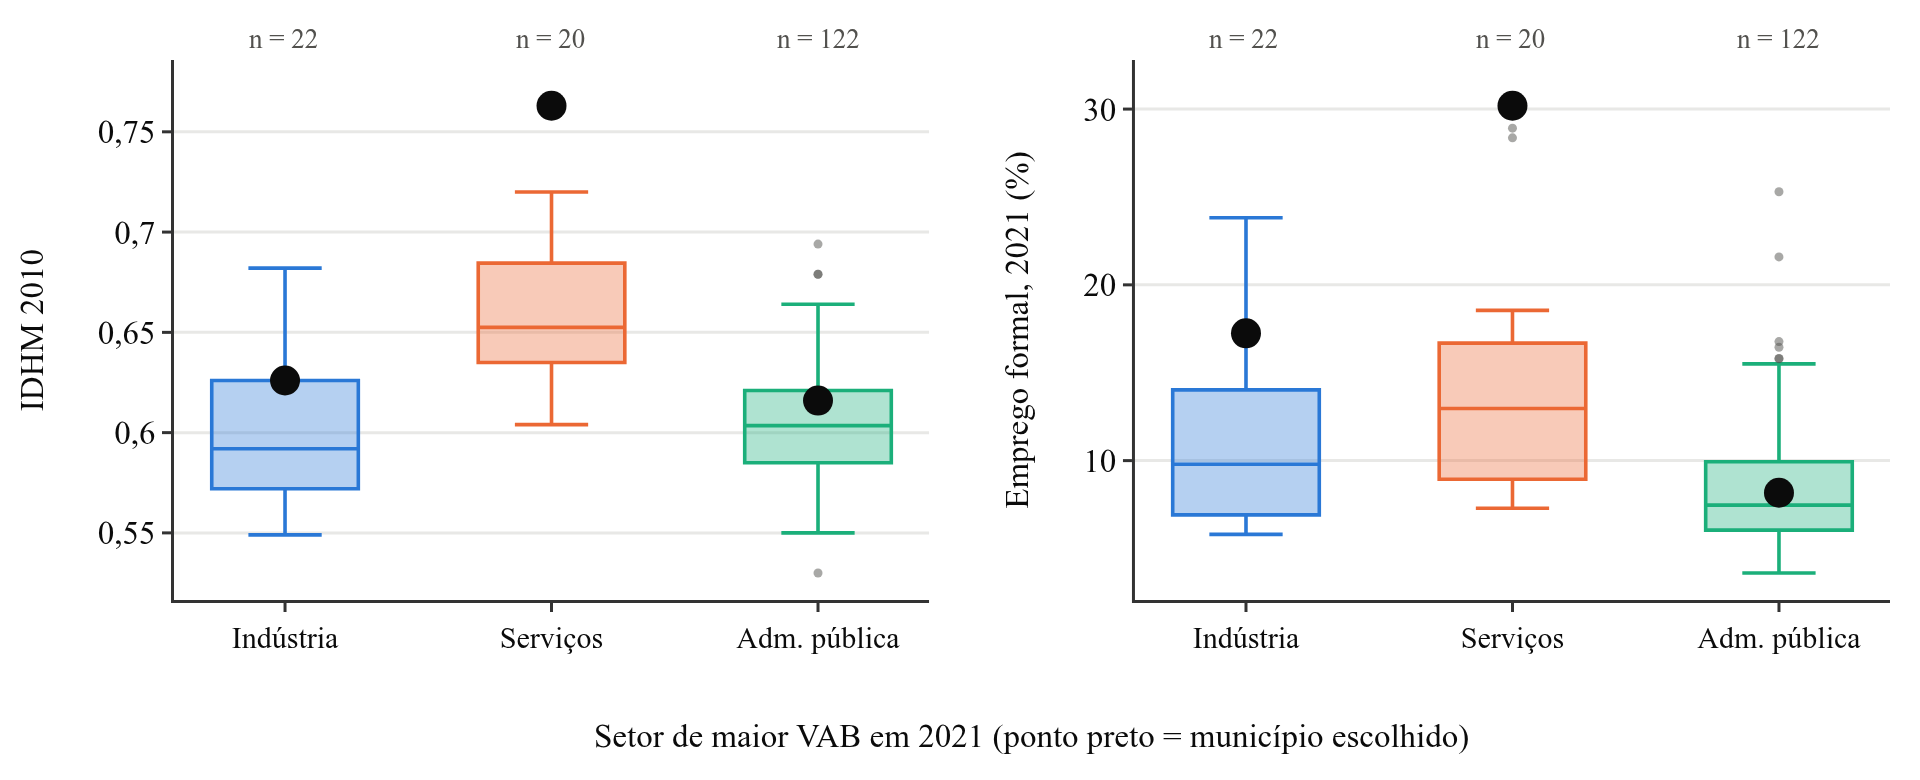
\includegraphics[width=0.9\textwidth]{fig5_adm_inversa.png}
\caption{IDHM (2010) e proporção da população em emprego formal (2021) segundo o setor de maior VAB do município em 2021 (164 municípios: omitidos os 3 em que nenhum dos três setores é o maior)}
\label{fig:inv}
\fonte{Fonte: elaborada pelo autor (2026) com dados do IBGE (2023), IBGE Cidades e CEMPRE 2021.}
\end{figure}


\subsection{Por que Guamaré, Natal e Ceará-Mirim}

``Alto VAB'' pode ser lido de três maneiras: VAB absoluto do setor (tamanho), participação do setor no VAB municipal (especialização) e VAB do setor por habitante. Os três municípios foram escolhidos por satisfazerem ao mesmo tempo quatro critérios: (i) estar entre os maiores do estado no VAB absoluto do setor; (ii) ter participação alta o bastante para caracterizar especialização; (iii) ter população suficiente para que os indicadores por habitante sejam estáveis; e (iv) dispor de literatura que permita identificar os fatores. A Tabela \ref{tab:rank} lista os cinco maiores de cada setor nos dois primeiros critérios e a Tabela \ref{tab:c} compara os escolhidos com o candidato mais forte de cada setor pelo critério de participação. A Figura \ref{fig:box} situa cada escolhido na distribuição do seu setor. Guamaré, com 75,0\% do VAB na indústria, está 3,2 desvios padrão acima da média (14,6\%; mediana 5,4\%), fora da caixa e entre os pontos extremos; Natal, com 64,2\% nos serviços, está 3,2 desvios padrão acima da média (28,3\%; mediana 26,3\%), também extremo; Ceará-Mirim, com 46,3\% na administração pública, está dentro da caixa (36,9\% a 62,7\%), um pouco abaixo da mediana (51,7\%) e da média (48,6\%): é o caso típico, não o extremo.

\begin{figure}[!htb]
\centering
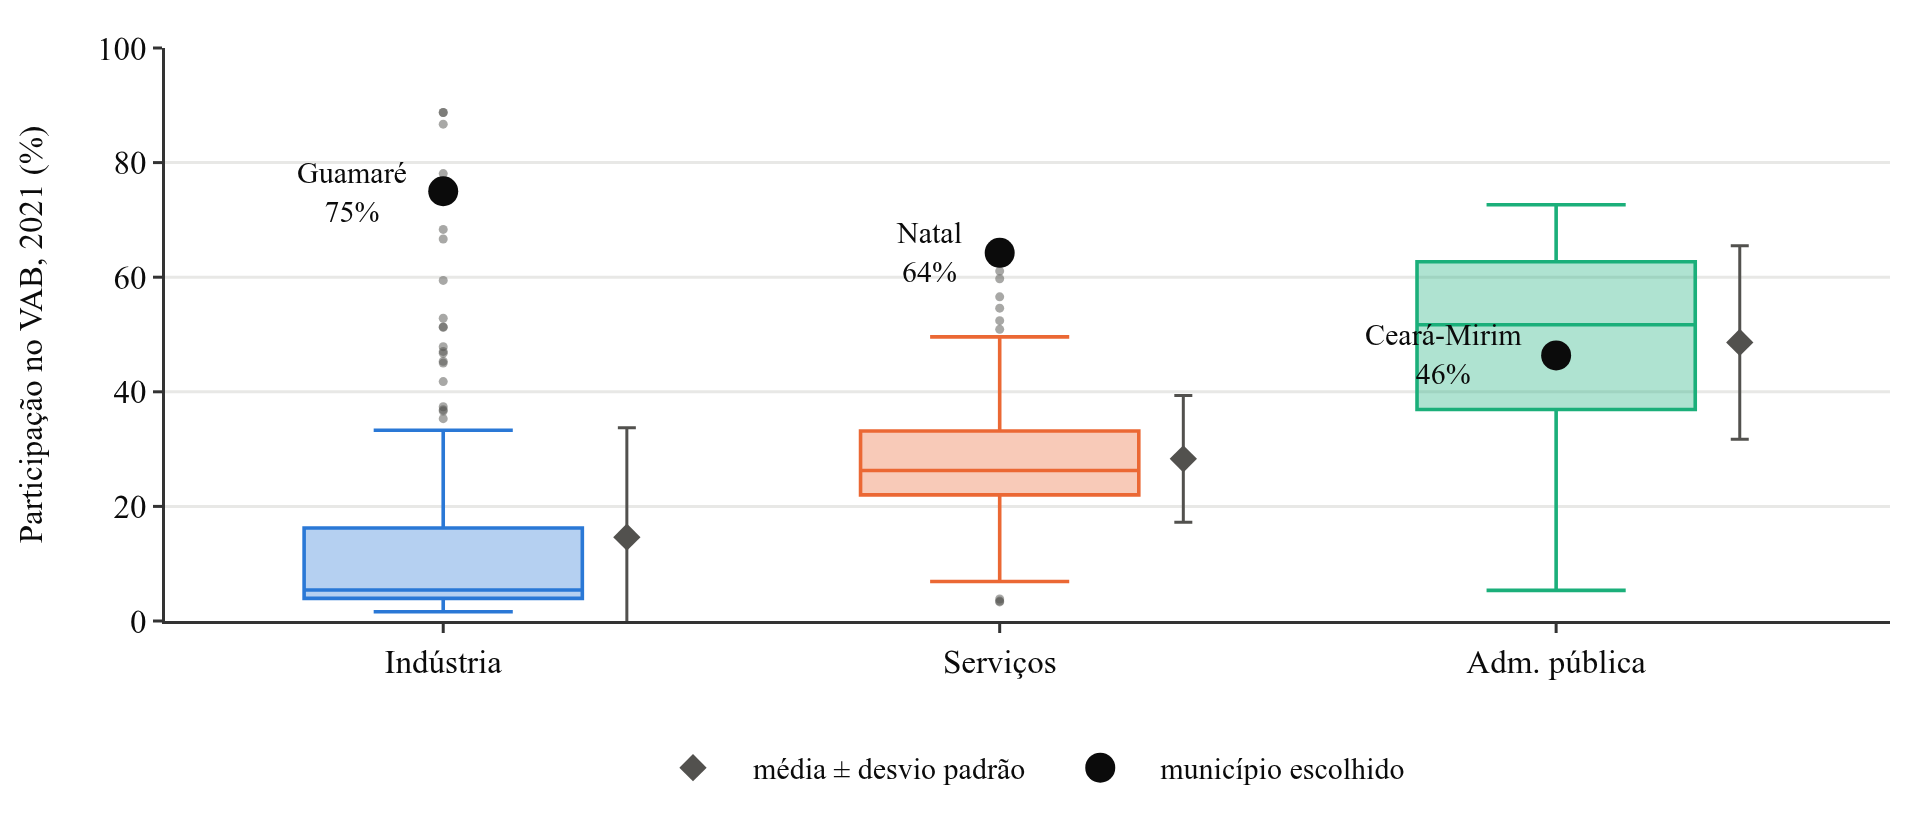
\includegraphics[width=0.8\textwidth]{fig1_boxplot.png}
\caption{Participação de cada setor-alvo no VAB municipal em 2021, 167 municípios: diagrama de caixa (mediana e quartis), média $\pm$ desvio padrão e município escolhido}
\label{fig:box}
\fonte{Fonte: elaborada pelo autor (2026) com dados do IBGE (2023).}
\end{figure}

\begin{table}[!htb]
\centering
\caption{Cinco maiores municípios de cada setor em 2021, por VAB absoluto e por participação no VAB municipal (VAB do setor em R\$ milhões; participação em \%)}
\label{tab:rank}
\footnotesize
\begin{tabular}{@{}c>{\raggedright\arraybackslash}p{6.6cm}>{\raggedright\arraybackslash}p{6.6cm}@{}}
\toprule
Pos. & Por VAB absoluto (VAB; part.) & Por participação (part.; VAB) \\
\midrule
\multicolumn{3}{@{}l}{\textit{Indústria}} \\
1º & Natal (2.557; 12,3) & São Bento do Norte (88,7; 452) \\
2º & \textbf{Guamaré} (1.471; 75,0) & Parazinho (88,7; 528) \\
3º & Mossoró (1.285; 18,6) & Bodó (86,7; 246) \\
4º & João Câmara (712; 59,4) & Pedra Grande (78,1; 213) \\
5º & Parnamirim (578; 10,2) & \textbf{Guamaré} (75,0; 1.471) \\
\midrule
\multicolumn{3}{@{}l}{\textit{Serviços}} \\
1º & \textbf{Natal} (13.348; 64,2) & \textbf{Natal} (64,2; 13.348) \\
2º & Mossoró (3.766; 54,6) & Pau dos Ferros (63,5; 389) \\
3º & Parnamirim (3.470; 61,1) & Parnamirim (61,1; 3.470) \\
4º & São Gonçalo do Amarante (878; 52,4) & Tibau do Sul (59,7; 228) \\
5º & Caicó (687; 56,6) & Caicó (56,6; 687) \\
\midrule
\multicolumn{3}{@{}l}{\textit{Administração pública}} \\
1º & Natal (4.851; 23,4) & João Dias (72,7; 20) \\
2º & Mossoró (1.663; 24,1) & Venha-Ver (72,4; 30) \\
3º & Parnamirim (1.550; 27,3) & Campo Redondo (71,0; 73) \\
4º & São Gonçalo do Amarante (589; 35,2) & Coronel João Pessoa (71,0; 33) \\
5º & Macaíba (433; 27,7) & Jundiá (70,8; 29) \\
\bottomrule
\end{tabular}
\fonte{Fonte: elaborada pelo autor (2026) com dados do IBGE (2023). Nota: Ceará-Mirim é o 6º em VAB absoluto da administração pública e o maior entre os 122 municípios em que o setor domina.}
\end{table}


\textbf{Guamaré} é o segundo maior VAB industrial do estado (R\$ 1,47 bilhão, 10,0\% do total potiguar), com 75,0\% do VAB no setor, 16.261 habitantes e literatura própria (Silva; Aquino, 2016); São Bento do Norte tem participação maior (88,7\%), mas VAB absoluto quatro vezes menor, 2.687 habitantes e nenhum estudo publicado. \textbf{Natal} é o primeiro em VAB de serviços (R\$ 13,35 bilhões, 41,3\% do estado) e em participação (64,2\%); Pau dos Ferros é o segundo em participação, mas o nono em VAB absoluto. \textbf{Ceará-Mirim} é o maior VAB da administração pública (R\$ 419 milhões, sexto do estado) entre os 122 municípios em que esse setor domina, com 46,3\% de participação e 74.268 habitantes; João Dias tem a maior participação (72,7\%), mas VAB vinte vezes menor e 2.653 habitantes. Ceará-Mirim é também típico (PIB per capita e IDHM a menos de 0,3 desvio padrão da média estadual): o que se diz dele vale para a maioria dos 122. Os fatores de cada caso vêm da literatura e dos dados. Guamaré: polo de refino e processamento de gás da Bacia Potiguar, operado pela Petrobras até a venda à 3R Petroleum em 2023 (Silva; Aquino, 2016; 3R Petroleum, 2023), regra do IBGE que aloca o VAB do petróleo nos municípios produtores e preço do petróleo, que tornou o VAB industrial negativo entre 2011 e 2014, quando o custo do insumo superou o valor da produção no refino (IBGE, 2015). Natal: função de capital, densidade e concentração do comércio, da saúde, da educação e da administração pública, no topo da rede urbana potiguar (Dantas; Clementino, 2014). Ceará-Mirim: declínio das usinas de açúcar e destilarias a partir da década de 1970, sem substituição industrial (Andrade, 2023), e população grande o bastante para que a folha pública seja a maior parcela da economia.

\begin{table}[!htb]
\centering
\caption{Municípios escolhidos e candidatos alternativos por setor, 2021 (posição entre os 167 municípios entre parênteses)}
\label{tab:c}
\footnotesize\setlength{\tabcolsep}{3pt}
\begin{tabular}{@{}>{\raggedright\arraybackslash}p{3.5cm}>{\centering\arraybackslash}p{1.6cm}>{\centering\arraybackslash}p{1.9cm}>{\centering\arraybackslash}p{1.6cm}>{\centering\arraybackslash}p{2.1cm}>{\centering\arraybackslash}p{2.0cm}>{\centering\arraybackslash}p{2.0cm}@{}}
\toprule
Município (setor) & População & VAB do setor (R\$ milhões) & Part. do setor no VAB (\%) & VAB do setor por habitante (R\$) & PIB per capita (R\$) & IDHM 2010 \\
\midrule
\textbf{Guamaré} (Ind.) & 16.261 & 1.471 (2º) & 75,0 (5º) & 90.463 (4º) & 125.585 (3º) & 0,626 (43º) \\
São Bento do Norte (Ind.) & 2.687 & 452 (11º) & 88,7 (1º) & 168.285 (1º) & 204.407 (1º) & 0,555 (162º) \\
\textbf{Natal} (Serv.) & 896.708 & 13.348 (1º) & 64,2 (1º) & 14.885 (3º) & 26.972 (21º) & 0,763 (2º) \\
Pau dos Ferros (Serv.) & 30.802 & 389 (9º) & 63,5 (2º) & 12.631 (6º) & 23.029 (32º) & 0,678 (10º) \\
\textbf{Ceará-Mirim} (Adm.) & 74.268 & 419 (6º) & 46,3 (101º) & 5.645 (152º) & 13.494 (83º) & 0,616 (63º) \\
João Dias (Adm.) & 2.653 & 20 (165º) & 72,7 (1º) & 7.473 (27º) & 10.551 (135º) & 0,530 (167º) \\
\midrule
Mediana dos 167 & 8.297 & --- & --- & --- & 13.469 & 0,606 \\
\bottomrule
\end{tabular}
\fonte{Fonte: elaborada pelo autor (2026) com dados do IBGE (2023) e IBGE Cidades. Nota: em negrito, os escolhidos; VAB por habitante = VAB do setor / população de 2021.}
\end{table}

\subsection{Vale a pena explorar Pau dos Ferros, João Dias e São Bento do Norte?}

Participação no VAB e VAB por habitante não contam a mesma história. Contra o PIB per capita, só a participação da indústria sobe ($b = 0{,}97$ mil reais por ponto percentual; são industriais 15 dos 17 municípios acima do P90 na Figura \ref{fig:sep}); a dos serviços desce levemente ($b = -0{,}68$), porque os municípios mais ricos são enclaves industriais com poucos serviços, e a da administração pública desce com clareza ($b = -0{,}91$), porque marca os mais pobres. Já o VAB do setor por habitante cresce com o PIB per capita nos três setores: na administração pública, os municípios pequenos recebem mais FPM por habitante e os petrolíferos financiam folhas maiores com royalties, e Guamaré é o segundo do estado nesse indicador (R\$ 11.731), contra o 152º lugar de Ceará-Mirim (R\$ 5.645).

Os três candidatos valem a pena, cada um por uma razão. \textbf{São Bento do Norte} é o caso-limite da indústria: primeiro em participação, em VAB industrial por habitante e em PIB per capita, e 162º em IDHM, o que torna o paradoxo de Guamaré ainda mais nítido; com 2.687 habitantes e sem literatura própria, serve para ilustrar, não para explicar. \textbf{Pau dos Ferros} é o contraponto a Natal: serviços sem função de capital, sustentados pelo comércio regional e por três instituições públicas de ensino superior, com VAB de serviços por habitante (R\$ 12.631) próximo ao da capital e IDHM entre os dez melhores (Dantas; Clementino, 2014); mostra que a associação entre serviços e IDHM não depende do tamanho da cidade. \textbf{João Dias} é o arquétipo da participação (72,7\%), e seu VAB da administração pública por habitante (R\$ 7.473) supera o de Ceará-Mirim e o de Natal, porque a cota do FPM por habitante é maior nos municípios pequenos; ainda assim, tem o pior IDHM do estado. A exploração é recomendável, desde que o VAB do setor por habitante acompanhe a participação e os 50 municípios com menos de 5 mil habitantes sejam tratados como casos ilustrativos.

\section{Diálogo com a literatura}

\subsection{Os dois artigos}

Mendes \textit{et al.} (2018) investigaram, com regressão logística em painel para os municípios brasileiros entre 2007 e 2013, a influência da capacidade econômica e das receitas públicas sobre a chance de o município alcançar Índice Firjan de Desenvolvimento Municipal (IFDM) de pelo menos 0,600, tendo como explicativas o PIB de cada setor (entre eles indústria e serviços), as receitas próprias e as transferências. O PIB da indústria teve o maior efeito positivo (razão de chances de 2,55); o PIB dos serviços foi ``a única variável aplicada ao modelo que apresentou efeito negativo''; e as transferências da União foram as mais relevantes, o que ``pode indicar dependência financeira desses recursos''; a conclusão é que ``o porte industrial [...] foi o de maior relevância para o desenvolvimento humano'' (Mendes \textit{et al.}, 2018, p. 929-931).

Fernandes, Tavares e Azevedo (2018), na RACE, estudaram os próprios municípios potiguares: com 166 municípios entre 2010 e 2013, explicaram o PIB municipal pelo VAB de cada setor, pelo IFDM e pela população. Todos os VAB setoriais tiveram efeito positivo e significativo (coeficientes entre 1,02 e 1,39) e o IFDM, sinal negativo; os autores concluem que o PIB mede crescimento, não qualidade de vida.

\subsection{O que os dados de 2021 comprovam}

O resultado de Fernandes, Tavares e Azevedo (2018) é comprovado de forma direta e com as ferramentas mais simples. A participação da indústria sobe com o PIB per capita, os 17 municípios acima do P90 são quase todos industriais e Natal, Mossoró e Parnamirim continuam somando quase metade do PIB estadual. Parte dessa relação é contábil, porque o PIB é a soma dos VAB mais os impostos; o que os dados acrescentam é a magnitude. O sinal negativo que os autores encontraram para o IFDM é coerente com a Tabela \ref{tab:p} e a Figura \ref{fig:inv}: os municípios mais ricos em PIB per capita não têm IDHM maior que os demais. A contradição entre VAB alto e desenvolvimento humano baixo, que os autores registram sem explicar, ganha aqui um mecanismo: nos municípios de enclave, o VAB é contabilizado no território, mas o lucro, os salários mais altos e os impostos federais são apropriados fora dele. Silva e Aquino (2016) já haviam mostrado, com dados de 2000 a 2011, que Guamaré tinha o maior PIB per capita do estado, mas IDHM abaixo da média estadual: o ``paradoxo do subdesenvolvimento com abundância de divisas''. Os dados de 2021 mostram que o paradoxo persiste e se estendeu aos municípios eólicos: Parazinho e São Bento do Norte, com 88,7\% do VAB na indústria, têm IDHM entre os seis piores do estado.

O resultado de Mendes \textit{et al.} (2018) sobre as transferências também é comprovado, desde que se distinga volume de dependência: elas sustentam quase todas as prefeituras potiguares (mediana de 91\% da receita), mas a dependência mais alta está no grupo abaixo do P10 (93,3\%), onde o emprego formal é menor e o IDHM é o pior. É o retrato que Gomes e Mac Dowell (2000) anteciparam, transferências pós-1988 que beneficiaram os pequenos municípios sem estimular sua produção, e que Araújo e Lima (2009) chamaram de ``economia sem produção''; Ceará-Mirim e os 122 municípios do mesmo perfil são sua expressão potiguar.

\subsection{O que os dados de 2021 contestam}

A conclusão de Mendes \textit{et al.} (2018) de que a indústria é o setor mais relevante para o desenvolvimento humano não se sustenta no Rio Grande do Norte. No Brasil, PIB industrial alto costuma significar indústria de transformação em cidades grandes, com empregos, fornecedores locais e serviços associados (encadeamentos). No Rio Grande do Norte, a participação industrial extrema ocorre em municípios pequenos com uma única planta de petróleo, sal ou energia eólica: o grupo acima do P90 tem mediana de 10.441 habitantes, 59,4\% do VAB na indústria e IDHM mediano de 0,605, igual ao do meio da distribuição. Parte da diferença é de medida: os autores usam o PIB setorial em nível, que cresce com o tamanho do município; este trabalho usa a participação, que mede especialização. A outra parte é de conteúdo: a indústria potiguar de maior VAB é extrativa e energética, sem os encadeamentos que o resultado nacional pressupõe.

O sinal negativo dos serviços encontrado por Mendes \textit{et al.} (2018), atribuído por eles a serviços de baixo valor agregado presentes em todos os municípios, também é contestado: nos dados potiguares a participação dos serviços é a variável mais associada ao IDHM (Figura \ref{fig:idhm}, painel central), e Natal, com 64\% do VAB em serviços, tem o segundo melhor IDHM do estado. A explicação provável está na classificação: no Rio Grande do Norte, o terciário de baixo valor agregado dos municípios pequenos aparece como administração pública, que o IBGE separa dos serviços; somada aos serviços, como em muitos estudos nacionais, ela puxa o coeficiente para baixo.

Em resumo, o que acontece em um município pode ser referenciado em outro de mesmo tipo, mas não entre tipos diferentes, distinção que um modelo nacional com todos os municípios não capta.

\section{Considerações finais}

Com média, desvio padrão, percentis e a reta $Y = a + bX$, foi possível identificar os fatores do alto VAB de Guamaré (polo de petróleo e gás, regra de alocação do VAB e preço do petróleo), de Natal (função de capital, densidade e concentração de serviços) e de Ceará-Mirim (declínio da cana e folha pública como base da economia) e justificar sua escolha frente a São Bento do Norte, Pau dos Ferros e João Dias. A reta, lida nos gráficos de dispersão, resumiu as relações sem o coeficiente de correlação: indústria e PIB per capita sobem juntos, indústria e IDHM não, serviços e IDHM sobem juntos, administração pública e emprego formal caminham em sentidos opostos. As separatrizes e os diagramas de caixa mostraram o paradoxo: Guamaré é extremo em renda e em participação industrial e mediano em desenvolvimento humano; Natal é extremo em serviços e em IDHM; Ceará-Mirim é o caso típico dos 122 municípios em que a prefeitura é a maior atividade, com IDHM menor e trabalho mais informal. O diálogo com Fernandes, Tavares e Azevedo (2018) e Mendes \textit{et al.} (2018) confirmou que VAB e PIB caminham juntos e contestou, para o caso potiguar, que a indústria seja o setor mais ligado ao desenvolvimento humano e que os serviços o prejudiquem: a medida (nível ou participação) e a classificação dos setores mudam o sinal das conclusões, o que recomenda cautela ao transferir resultados nacionais para um estado cuja indústria é de enclave.

Os achados se resumem em três observações. Primeira: no Rio Grande do Norte, indústria não significa desenvolvimento socioeconômico. Os municípios mais industriais são enclaves pequenos de petróleo, gás, sal e energia eólica, que ocupam o topo do PIB per capita (15 dos 17 acima do P90) mas têm o menor IDHM mediano entre os grupos setoriais (0,592), e a reta da indústria contra o IDHM é praticamente horizontal ($b = -0{,}003$). Segunda: os serviços são o setor mais associado ao desenvolvimento, o único cuja reta sobe com o IDHM ($b = +0{,}208$); os 20 municípios em que dominam têm o maior IDHM mediano (0,653) e o maior emprego formal (13,0\%), de Natal a Pau dos Ferros. Terceira: a administração pública é a moda do estado, o setor de maior VAB em 122 dos 167 municípios (73,1\%), e esse perfil, em que a prefeitura sustentada por transferências é a principal atividade econômica, vem acompanhado de IDHM mediano de 0,603 e de apenas 7,5\% da população em emprego formal. A estrutura econômica predominante no estado é, portanto, a da ``economia sem produção (Araújo; Lima, 2009), e é sobre ela, mais do que sobre a indústria, que políticas de desenvolvimento municipal no Rio Grande do Norte precisam atuar.

\section*{REFERÊNCIAS}
\begin{referencias}

3R PETROLEUM ÓLEO E GÁS S.A. \textbf{Fato relevante}: conclusão da aquisição do Polo Potiguar. Rio de Janeiro: 3R Petroleum, 7 jun. 2023. Disponível em: \url{https://api.mziq.com/mzfilemanager/v2/d/55b913af-cd4c-48d5-bc19-48c63916b8a5/56bf8b8b-7ebd-c7dd-e0a9-f31d07f5c7da}. Acesso em: 10 out. 2026.

ANDRADE, Manuel Correia de. As usinas de açúcar e as destilarias de álcool do Rio Grande do Norte. \textbf{Revista GeoInterações}, Assú, v. 7, e11, p. 175-185, 2023. Disponível em: \url{https://periodicos.apps.uern.br/index.php/RGI/article/view/5500}. Acesso em: 10 out. 2026.

ARAÚJO, Leonardo Alves de; LIMA, João Policarpo Rodrigues. Transferências de renda e empregos públicos na economia sem produção do semiárido nordestino. \textbf{Planejamento e Políticas Públicas}, Brasília, n. 33, p. 45-77, jul./dez. 2009. Disponível em: \url{https://repositorio.ipea.gov.br/bitstream/11058/3993/2/PPP_n33_Transferencias.pdf}. Acesso em: 10 out. 2026.


DANTAS, Joseney Rodrigues de Queiroz; CLEMENTINO, Maria do Livramento Miranda. Desenvolvimento e urbanização: a rede urbana potiguar sob a ótica dos ``REGICs''. \textbf{Geotemas}, Pau dos Ferros, v. 4, n. 1, p. 71-82, jan./jun. 2014. Disponível em: \url{https://periodicos.apps.uern.br/index.php/GEOTemas/article/view/606}. Acesso em: 10 out. 2026.

FERNANDES, Ruhama Bezerra; TAVARES, Adilson de Lima; AZEVEDO, Yuri Gomes Paiva. Relação entre o valor adicionado das atividades econômicas e o Produto Interno Bruto do Rio Grande do Norte. \textbf{RACE: Revista de Administração, Contabilidade e Economia}, Joaçaba, v. 17, n. 2, p. 757-782, maio/ago. 2018. DOI: 10.18593/race.v17i2.17238.

GOMES, Gustavo Maia; MAC DOWELL, Maria Cristina. \textbf{Descentralização política, federalismo fiscal e criação de municípios}: o que é mau para o econômico nem sempre é bom para o social. Brasília: IPEA, 2000. (Texto para Discussão, n. 706). Disponível em: \url{http://repositorio.ipea.gov.br/handle/11058/2339}. Acesso em: 10 out. 2026.

IBGE. \textbf{Produto interno bruto dos municípios 2013}: apresentação da divulgação. Rio de Janeiro: IBGE, Coordenação de Contas Nacionais, 18 dez. 2015. Disponível em: \url{https://anda.ibge.gov.br/media/com_mediaibge/arquivos/d7449516f181496dbff2a68cfdd9c349.pdf}. Acesso em: 10 out. 2026.

IBGE. \textbf{Produto interno bruto dos municípios}: ano de referência 2010. 3. ed. Rio de Janeiro: IBGE, 2016. (Relatórios Metodológicos, v. 29). Disponível em: \url{https://biblioteca.ibge.gov.br/visualizacao/livros/liv97483.pdf}. Acesso em: 10 out. 2026.

IBGE. \textbf{Produto interno bruto dos municípios 2021}: notas técnicas. Rio de Janeiro: IBGE, 2023. (Contas Nacionais, n. 96). Disponível em: \url{https://biblioteca.ibge.gov.br/visualizacao/livros/liv102057_notas_tecnicas.pdf}. Acesso em: 10 out. 2026.

IBGE. \textbf{Produto interno bruto dos municípios}: Brasil: 2022-2023: notas técnicas. Rio de Janeiro: IBGE, 2025. (Contas Nacionais, n. 104). Disponível em: \url{https://biblioteca.ibge.gov.br/visualizacao/livros/liv102250_notas_tecnicas.pdf}. Acesso em: 10 out. 2026.

MENDES, Wesley de Almeida; FERREIRA, Marco Aurélio Marques; ABRANTES, Luiz Antônio; FARIA, Evandro Rodrigues de. A influência da capacidade econômica e da formação de receitas públicas no desenvolvimento humano. \textbf{Revista de Administração Pública}, Rio de Janeiro, v. 52, n. 5, p. 918-934, set./out. 2018. DOI: 10.1590/0034-761220170004.


SILVA, Maria Russilânya Costa Santos da; AQUINO, Joacir Rufino de. Subdesenvolvimento humano com abundância de riqueza: o caso dos ``municípios petrorrentistas'' do Rio Grande do Norte. \textbf{Revista GeoNordeste}, São Cristóvão, ano 27, n. 1, p. 71-91, jan./jul. 2016. Disponível em: \url{https://periodicos.ufs.br/geonordeste/article/view/4572}. Acesso em: 10 out. 2026.

\end{referencias}
\end{document}
